\documentclass[
% twocolumn,
% hf,
]{ceurart}
%%
%% One can fix some overfulls
\sloppy

%%
%% Minted listings support 
%% Need pygment <http://pygments.org/> <http://pypi.python.org/pypi/Pygments>
\usepackage{listings}
%% auto break lines
\lstset{breaklines=true}


% \usepackage[T1]{fontenc}
\usepackage{graphicx}
% \usepackage[caption=false]{subfig}
% \usepackage{amsmath, amssymb}
% \usepackage{bm}
% \usepackage{float}

\usepackage{xcolor}
\newenvironment{zholtkevych}{\color{red}}{}
\newenvironment{review}{\color{blue}}{}
\newenvironment{old}{\color{gray}}{}

\newcommand{\todo}[1]{\textcolor{red}{[TODO:\@#1]}}

\begin{document}

% ===========================

%%
%% Rights management information.
\copyrightyear{2025}
\copyrightclause{Copyright for this paper by its authors.
  Use permitted under Creative Commons License Attribution 4.0
  International (CC BY 4.0).}

%%
%% This command is for the conference information
\conference{ProfIT AI'25: 5th International Workshop of IT-professionals on Artificial Intelligence,
  October 15--17, 2025, Liverpool, UK}

%%

%%
%% The "author" command and its associated commands are used to define
%% the authors and their affiliations.
\author[1]{Yurii Lytvynenko}[%
orcid=0009-0004-0732-0602, % chktex 8
email=inbox@yury-lytvynenko.com,
% url=https://yury-lytvynenko.com,
]
\cormark[1]
\fnmark[1]

\author[1,2]{Grygoriy Zholtkevych}[%
orcid=0000-0002-7515-2143, % chktex 8
email={g.zholtkevych@karazin.ua,grygoriy.zholtkevych@lnu.edu.ua}
% url=https://kmitd.github.io/ilaria/,
]
\fnmark[1]
\address[1]{V.N. Karazin Kharkiv National University,
  4 Svobody sq., Kharkiv, 61022, Ukraine}
\address[2]{Ivan Franko National University of Lviv,
  1 Universyteska Str., Lviv, 79007, Ukraine}

%% Footnotes
\cortext[1]{Corresponding author.}
\fntext[1]{These authors contributed equally.}

% ===========================


%% The "title" command
\title{Selecting a Simulation Runtime for Opinion Dynamics: Evaluating Elixir for Agent-Based Models}
% Elixir as a Runtime for Opinion Dynamics Simulations: Concurrency, Determinism, and Performance
% Concurrency-First Simulation of Networked Communities: Comparing Elixir and Python
% Scalable Simulation of Pairwise Communication Models Using the BEAM Virtual Machine
% Robust and Deterministic Opinion Dynamics Simulation with Elixir


\begin{abstract}
We evaluate Elixir as a simulation runtime for opinion dynamics by implementing the same extended pairwise dialogue model in three engines with RNG parity: an Elixir \emph{actor} engine, an Elixir \emph{task} engine, and a Python \emph{multiprocessing} baseline, ensuring identical outputs given the same seed. On a dense all-pairs stress test (\(N{=}300\), \(T{=}100\), \(\sim\)4.5M dialogues), the \emph{actor} engine was fastest; under a sparse random-matching topology (\(k{=}8\); 120k dialogues) the \emph{task} engine outperformed \emph{actor} by \(\approx\)18\%. Both Elixir engines consistently exceeded Python. Ten repeated trials produced tight 95\% confidence intervals, confirming stability and efficient multicore utilization on BEAM. We conclude that Elixir is a robust choice for high-concurrency agent-based simulations, with topology guiding engine selection (actor for dense, task for sparse). This runtime decision provides the methodological foundation for our subsequent modeling work.
\end{abstract}

\begin{keywords}
Opinion Dynamics \sep{} 
Agent-Based Simulation \sep{}
Simulation Runtime Evaluation \sep{} 
Elixir Programming Language \sep{} 
BEAM Virtual Machine \sep{} 
Computational Social Science \sep{} 
Methodological Foundations
\end{keywords}

\maketitle

\section{Introduction}
Simulation of opinion dynamics in networked communities is a computationally demanding task. Modern models, such as the extended pairwise dialogue framework~\cite{Lytvynenko2025}, represent social interactions as repeated dialogues where agents retain, adopt, or reject opinions based on attributes like resistance and persuasiveness. These models are mathematically rigorous and offer valuable insights into polarization, consensus, and the emergence of alternative viewpoints. However, their computational cost increases rapidly with network size and interaction density.

Selecting an appropriate programming language and runtime environment is therefore critical. The requirements are precise: the simulation must support a large number of lightweight, independent computations, manage concurrency efficiently, and scale across modern multicore processors without significant programmer overhead. While Python is traditionally used in computational social science due to its extensive ecosystem of scientific libraries, its concurrency limitations pose non-trivial challenges for such workloads.

Other languages have also been employed for computational modeling. Julia~\cite{Julia2025} offers high numerical performance and a growing ecosystem for scientific computing. However, its concurrency model is still evolving and less mature for large-scale distributed workloads. C and C++ deliver raw performance but require significant manual management of parallelism, memory, and fault tolerance, which increases development complexity and reduces flexibility. In contrast, Elixir~\cite{Elixir2025}, built on the Erlang virtual machine (BEAM)~\cite{Erlang2025}, provides a concurrency-first design. Its lightweight process model, supervision trees, and fault-tolerant architecture were created for large-scale distributed systems and map naturally onto multi-agent simulations where thousands of dialogues coincide.

In this paper, we argue that Elixir offers unique advantages as the core simulation engine for opinion dynamics models. By evaluating the extended dialogue model in the challenging setting of $N = 300$ agents under all pairs mode, we demonstrate that Elixir provides a scalable and robust foundation for simulation backends in computational social science. Importantly, this evaluation is not an end in itself but a methodological step: it was undertaken to identify the most suitable runtime for subsequent research on the dynamics of community opinions, where the extended dialogue model will be developed and applied at scale.

\section{Background}\label{sec:background}
\subsection{Opinion Dynamics Model}
The study of opinion dynamics seeks to understand how individual preferences evolve through repeated interactions within a community. In the extended dialogue model~\cite{Lytvynenko2025}, communication is represented as a series of \textbf{pairwise dialogues}. Each dialogue is treated as an atomic operation, where two agents exchange views and update their opinions probabilistically.

Unlike classical binary models, where agents either retain or adopt an interlocutor’s opinion, the extended framework introduces a third possibility: selecting an alternative state. As a result, each dialogue may lead to one of three outcomes:
\begin{enumerate}
	\item An agent retains their current opinion.
	\item An agent adopts the interlocutor’s opinion.
	\item An agent rejects both options and transitions to a generalized alternative.
\end{enumerate}
The likelihood of these outcomes is shaped by two independent attributes: \textbf{resistance} (the tendency to keep one’s own opinion) and \textbf{persuasiveness} (the ability to influence others). By decoupling these factors, the model captures more nuanced dynamics than deterministic consensus frameworks. For instance, when both agents exhibit high resistance and high persuasiveness, they may fail to persuade each other and instead converge on an alternative, reflecting real-world behaviors such as withdrawal from mainstream positions.

By explicitly modeling \textbf{resistance} and \textbf{persuasiveness} as independent attributes, the framework allows for richer dynamics than deterministic consensus models. For example, when both agents are highly resistant and highly persuasive, they may converge not on each other’s opinions but on an alternative, reflecting real-world behaviors such as rejection of mainstream narratives.


\subsection{Markovian Transition Structure}
The dialogue process is formalized as a Markov chain. Each pair of interacting agents constitutes a state, defined by their current opinions. Transition probabilities between states are governed by the agents' resistance ($\rho$) and persuasiveness ($\pi$) values. This leads to a stochastic transition matrix $T$, where each row sums to one and encodes the likelihood of moving from one dialogue outcome to another.

The Markovian structure ensures that opinion evolution is both mathematically tractable and computationally efficient to implement, while still capturing non-trivial behaviors such as deadlocks, polarization, or convergence to alternatives.


\subsection{Computational Requirements}
Although conceptually simple, the extended dialogue model, where opinion updates occur through pairwise dialogues, becomes computationally demanding at scale. Suppose a network has $N$ agents and, in each iteration, every agent engages in $k$ dialogues with distinct peers (assuming dialogues are undirected):

\[
D(N,k)=\frac{N\,k}{2}
\]

Over $T$ iterations, the total number of dialogue computations is $T \cdot D$. Each dialogue triggers a probabilistic state update governed by the model's transition rules, so runtime scales with both $N$ and $k$, and $T$.

To illustrate, consider a sizeable community with $N=100{,}000$ agents where each agent interacts with $k=20$ distinct peers per iteration (e.g., a dense social platform cohort or an enterprise communication snapshot). Then:

\[
D(100{,}000,20)=\frac{100{,}000 \times 20}{2}=1{,}000{,}000
\]

dialogues \textbf{per iteration}. Across $T=1{,}000$ iterations, that yields

\[T \cdot D=1{,}000 \times 1{,}000{,}000=10^{9}\]

dialogues --- each an independent, lightweight computation whose outcomes must be aggregated into consistent agent states for the next iteration. This profile highlights three practical demands:
\begin{itemize}
	\item \textbf{High volume of independent interactions} (embarrassingly parallel within an iteration);
	\item \textbf{Natural concurrency} (amenable to multi-core and distributed execution);
	\item \textbf{State management pressure} (efficient aggregation and deterministic progression across iterations).
\end{itemize}

This workload profile requires a runtime capable of handling massive concurrency with minimal overhead while maintaining robustness over extended execution times.

\section{Elixir as a Simulation Runtime}

\textbf{Elixir}, a functional programming language built on the Erlang virtual machine (BEAM)~\cite{Elixir2025}, was designed originally for distributed, fault-tolerant systems. Its lightweight process model, supervision trees, and transparent scalability across multicore and distributed environments directly address the requirements identified in Section~\ref{sec:background}. These features make Elixir a natural fit for implementing large-scale opinion dynamics simulations in computational social science.

\subsection{Concurrency Model}
Elixir implements the actor model through lightweight processes that communicate via message passing. These processes are inexpensive to create and schedule, enabling thousands to run simultaneously on a single machine. In the context of opinion dynamics, this allows each agent or dialogue to be represented as an isolated process, mirroring the independence of interactions in the model. The result is a natural mapping between simulation logic and execution.

\subsection{Fault Tolerance}
Long-running simulations can be disrupted by runtime errors, leading to incomplete or inconsistent results. Elixir addresses this with supervision trees, which monitor groups of processes and automatically restart them in case of failure. This design provides resilience without requiring explicit error-handling logic for every component, ensuring that simulations can run reliably over millions of dialogue steps.

\subsection{Distribution}
The BEAM runtime also supports transparent distribution, allowing processes to span multiple CPU cores or even multiple machines with minimal configuration changes. Since dialogues are independent, distributing them across cores or nodes is straightforward, enabling simulations to scale horizontally as network size or iteration count increases.

\subsection{Comparison to Python}
Python remains the default language for computational modeling due to its extensive scientific libraries and user-friendly syntax. However, its runtime is poorly suited for workloads dominated by massive concurrency:

\begin{itemize}
	\item The Global Interpreter Lock (GIL) prevents true parallel execution of threads on multiple cores.~\cite{PythonThreading}
	\item Achieving parallelism typically requires additional frameworks such as \emph{multiprocessing}~\cite{PythonMultiprocessing}, \emph{Dask}~\cite{PythonDask}, or \emph{Ray}~\cite{PythonRay}, which add overhead and complexity.
	\item Fault tolerance and process supervision must be implemented manually, increasing the risk of brittle long-running simulations.
\end{itemize}

Elixir integrates concurrency, fault tolerance, and distribution at both the language and runtime level. These properties make it particularly well-suited for large-scale opinion dynamics simulations, where each iteration involves thousands or even millions of independent dialogues across a network. By reducing implementation complexity and minimizing runtime overhead, Elixir offers a compelling alternative to Python for executing the simulation core, particularly in scenarios that require sustained high concurrency and reliable long-running performance.

It is worth noting that recent developments in Python (PEP 703)~\cite{pep703} have introduced a no-GIL build, which allows for true parallelism across threads. While promising, this feature is not yet the default in production environments, lacks broad library support, and was therefore excluded from our evaluation. We restrict our comparison to the widely used mainstream Python runtime, which remains the de facto standard in computational social science.



\section{Experimental Comparison of Elixir and Python}
Based on the requirements and architectural considerations outlined in the previous sections, we did an empirical comparison of Elixir and Python. The goal of these experiments was not to fine-tune implementations, but rather to observe how the two runtimes handle workloads characterized by large numbers of lightweight, independent interactions. Both languages were used to execute the same extended dialogue model under identical simulation parameters, enabling a direct assessment of concurrency handling, scalability, and robustness.

\subsection{Simulation Parameters}
\begin{itemize}
    % \item \textbf{Network size (\textbf{N})}: 200 agents.
	\item \textbf{Interaction pattern}: \emph{all pairs} — every agent interacts with every other agent in each iteration. Although this pattern may not be realistic, it is employed as a worst-case stress test to maximize computational load while keeping the model simple. By adopting the all-pairs setup, we avoid additional complexity related to dynamically selecting subsets of peers and ensure that differences in runtime performance can be attributed directly to the efficiency of the execution environment.

	\item \textbf{Total dialogues per iteration}:
$D(N) = \binom{N}{2} = \frac{N(N-1)}{2}$
For $N = 300$, this results in $44{,}850$ dialogues per iteration.
	\item \textbf{Iterations (T)}: 100.
	\item \textbf{Attributes}: Each agent is initialized with random values of resistance ($\rho \in [0,1]$) and persuasiveness ($\pi \in [0,1]$) drawn from a uniform distribution.
	\item \textbf{Outcome aggregation}: Dialogue outcomes are accumulated per agent and averaged at the end of each iteration to update preferences.
\end{itemize}


\subsection{Experimental Environment}
All experiments were conducted on a dedicated Amazon EC2 instance of type \textbf{c8g.2xlarge}~\cite{AwsInstanceTypes2025}, equipped with \textbf{8 vCPUs} and \textbf{16 GiB RAM}, based on the \textbf{AWS Graviton3 (ARM64) architecture}. The instance was located in the \textbf{us-east-1 region}. CPU frequency scaling was left at the AWS defaults (no explicit pinning to performance mode).

The operating system was \textbf{Ubuntu 24.04 LTS} with kernel version \textbf{6.14.0-1011-aws}.% chktex 8

The software stack included:
\begin{itemize}
    \item \textbf{Elixir 1.14.0} (compiled with Erlang/OTP 24), running on \textbf{Erlang/OTP 25 [erts-13.2.2.5]} with JIT enabled.
    \item \textbf{Python 3.12.3}, installed via the system package manager (apt).
    \item No external Python packages were required beyond the standard library.
\end{itemize}

Both implementations were installed from Ubuntu's package repositories (apt) to ensure a consistent and reproducible setup.


The benchmarks were run on a \textbf{dedicated instance} without competing workloads.

\subsection{Implementations}
To run the experiments, we developed three independent implementations of the extended dialogue model: two in Elixir and one in Python. Although they differ in architecture and concurrency approach, they all adhere to the same specification to guarantee deterministic parity of results. Shared design choices include:

\begin{itemize}
	\item \textbf{All-pairs interaction} at each iteration, with agent indices ordered ($i < j$) to enforce consistency in dialogue roles.
	\item \textbf{Random number generation (RNG) parity} through a shared 64-bit Linear Congruential Generator (LCG)~\cite{Thomson1958}, seeded identically and consumed in the same order across engines.
	\item \textbf{Aggregation} by summing contributions per agent and dividing by $N-1$.
	\item \textbf{Rounding} to three decimals at fixed stages, ensuring identical numeric results across languages.
\end{itemize}

It was explicitly validated that all three implementations return identical results given the same parameters and seed, confirming that observed differences in performance are due solely to runtime characteristics rather than algorithmic divergence. Validation was performed by cross-checking outputs across engines, including per-agent preference vectors, average preferences, and vote distributions, ensuring complete agreement within rounding precision.

\subsubsection{Elixir Task Engine}
Uses \verb|Task.async_stream| to parallelize batches of pairwise dialogues. Each iteration generates all pairs, divides them into chunks, processes them concurrently, and then reduces the results to update agents' states.

\subsubsection{Elixir Actor Engine}
Implements an actor-based design, with one process per agent and a central Coordinator. Each iteration begins with a snapshot of agent states stored in ETS.\@Agent processes compute contributions against their peers and send results back to the Coordinator, which merges them and updates agent states.

\subsubsection{Python Multiprocessing Engine}
Mirrors the Elixir Task Engine design, utilizing the multiprocessing module. Pairs are generated with $i < j$, partitioned into chunks, and distributed to worker processes. Results are collected, reduced per agent, and averaged.


\subsection{Execution Time and Community Size}
To assess scalability, we measured execution time as the simulated community size increased, using the \emph{all pairs} interaction pattern for 100 iterations.

We report results starting from $N=100$. Below this threshold, the number of dialogues per iteration is too small to produce meaningful performance comparisons, as runtimes are dominated by fixed overhead. At $N=100$, however, each iteration already requires 4,950 dialogues, yielding nearly half a million dialogues across the experiment, which is a substantial computational load.

Execution time grows in line with the quadratic complexity of the all-pairs configuration ($\binom{N}{2}$), but the rate and pattern of growth differ across implementations:

\begin{itemize}
\item \textbf{Elixir Actor Engine} consistently delivers the best results across all tested community sizes. Despite the coordination overhead of its GenServer design, it handles scaling more efficiently, leading to lower execution times throughout.
\item \textbf{Elixir Task Engine} performs well but is outpaced by the Actor engine even at small sizes, suggesting that its task scheduling overhead accumulates less favorably.
\item \textbf{Python multiprocessing} lags significantly behind both Elixir implementations. The gap widens with larger N, reflecting the steep cost of inter-process communication and serialization.
\end{itemize}

\begin{figure}
  \centering
  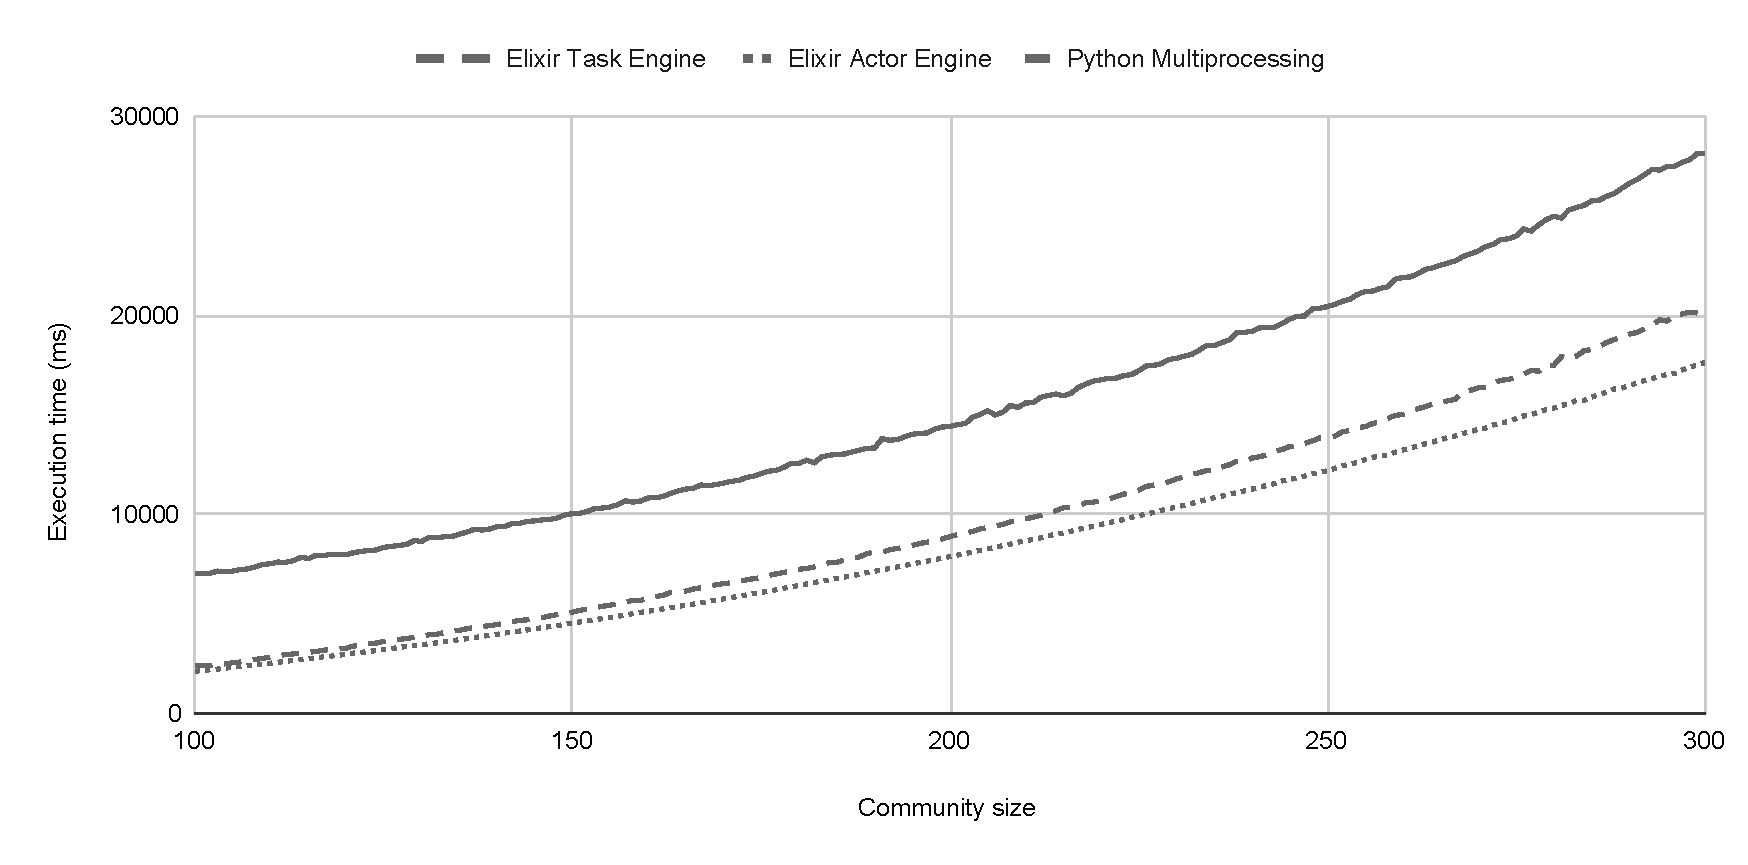
\includegraphics[width=\linewidth]{images/wall_time_community_100-300.pdf} % chktex 8
  \caption{Execution time (ms) for 100 iterations of the all-pairs interaction model as a function of community size N}
\end{figure}

\subsubsection{Throughput Analysis}

In addition to raw execution time, it is instructive to examine throughput, measured as the number of dialogues processed per second. Throughput was computed as:

\[\text{Throughput} = \frac{\text{Total dialogues}}{\text{Execution time (s)}}\]

where the total dialogues equal the number of iterations (T = 100) multiplied by $\binom{N}{2}$, and execution time was measured in milliseconds and converted to seconds.

Across all tested community sizes, \textbf{Elixir Actor Engine} consistently achieves the highest throughput, surpassing both Elixir Task Engine and Python. While Elixir Task Engine performs well, it is outpaced by the Actor engine, indicating that the GenServer-based design not only scales better but also processes dialogues faster in absolute terms. Python multiprocessing lags substantially behind, reflecting the cost of inter-process communication and serialization overhead.

\begin{figure}
  \centering
  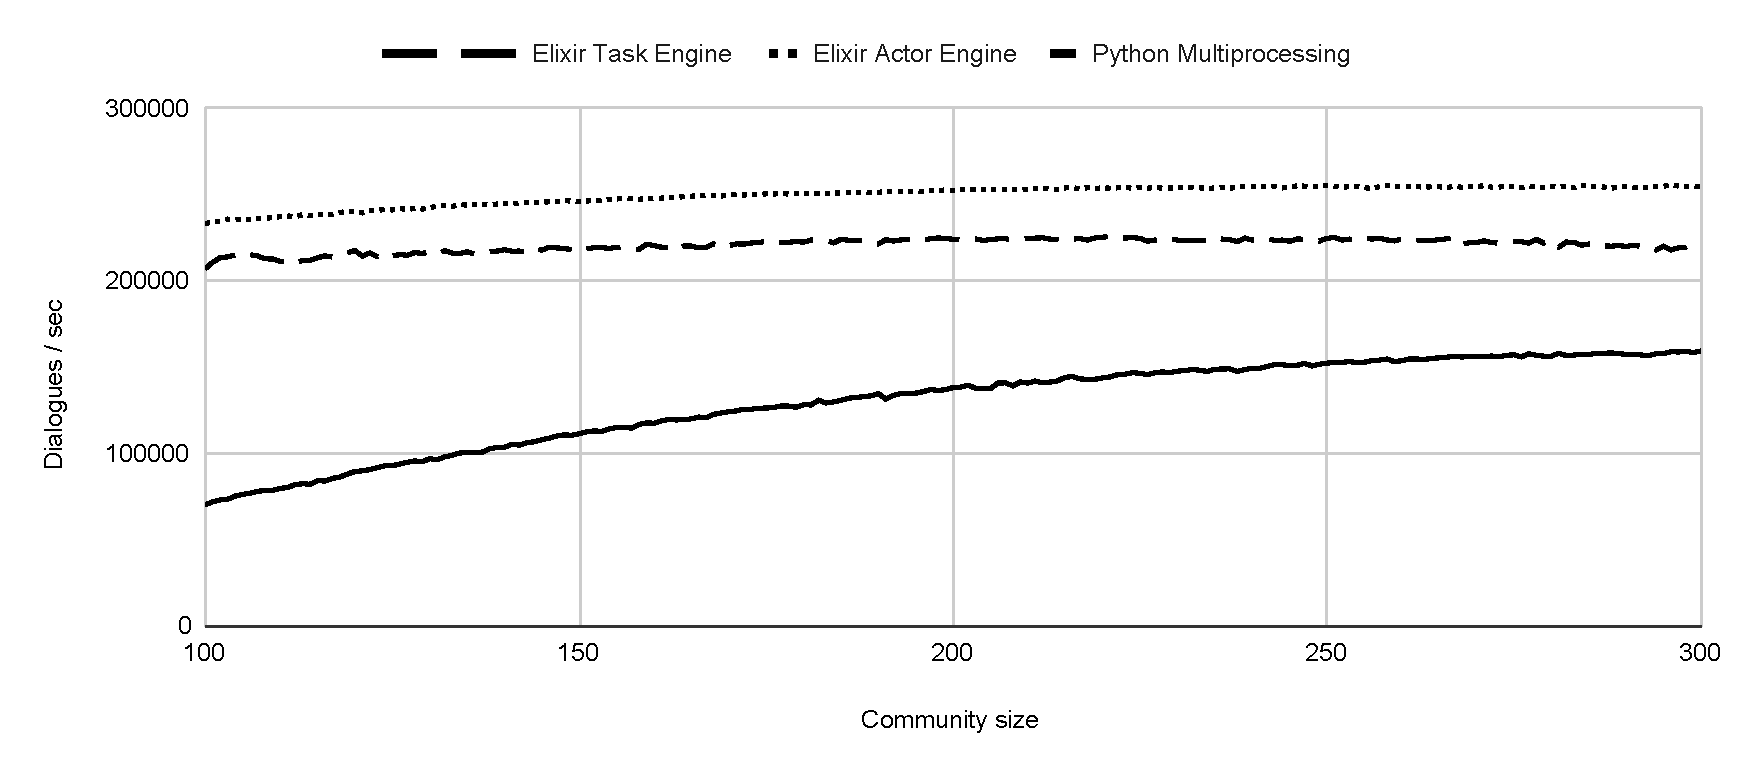
\includegraphics[width=\linewidth]{images/throughput_community_100-300.pdf} % chktex 8
  \caption{Throughput (dialogues/sec) for 100 iterations under all-pairs interaction, as a function of community size N}
\end{figure}


It should be noted that these measurements are based on \textbf{single runs per configuration}. While absolute values may vary across repeated executions, the observed ordering of performance and relative scaling trends provide clear evidence of Elixir's advantage as a simulation runtime.


\subsection{Repeated Trials at Fixed Parameters}
Having established how execution time scales with community size, we next examine performance under fixed parameters by conducting repeated trials. This setting provides a complementary view, focusing on the stability and relative efficiency of the three implementations when the workload is held constant.

\subsubsection{Benchmarking Methodology}
To ensure reliable and reproducible performance measurements, we developed a systematic benchmarking infrastructure. The methodology consists of three components:

\textbf{Resource Monitoring.} Each simulation run is monitored using the Python \texttt{psutil} library~\cite{PythonPsutil}, which tracks the entire process tree (parent and all child processes). Three metrics are collected:
\begin{itemize}
	\item \textbf{Wall-clock time} (ms): total elapsed time from process start to completion;
	\item \textbf{Peak memory usage} (KB): maximum resident set size (RSS) across the process tree;
	\item \textbf{Average CPU utilization} (\%): mean CPU usage measured as system-wide CPU percentage scaled by core count, representing the effective parallelization (e.g., 800\% indicates full utilization of 8 cores).
\end{itemize}

Metrics are sampled at 100ms intervals throughout execution. Memory is tracked per-process and summed across all descendants to capture the full resource footprint of concurrent implementations.

\textbf{Statistical Analysis.} Raw benchmark data from multiple trials are aggregated using a bootstrap method~\cite{Efron1979} to compute robust confidence intervals. For each metric and configuration, we calculate:
\begin{itemize}
	\item \textbf{Median}: the central tendency, robust to outliers;
	\item \textbf{95\% confidence interval}: derived from 10,000 bootstrap samples with replacement, providing upper and lower bounds on the median estimate.
\end{itemize}

This approach avoids distributional assumptions and provides reliable interval estimates even with small sample sizes (n=10 trials).

\textbf{Execution Control.} Benchmarks are orchestrated by shell scripts that execute each configuration multiple times with identical parameters (agents, iterations, seed, chunk size). Results are recorded in CSV format with one row per trial, enabling reproducibility and subsequent statistical analysis. All benchmarks were run on an isolated AWS EC2 instance (c8g.2xlarge, ARM64) without competing workloads to minimize measurement noise.

\subsubsection{All-Pairs Topology Results}
The configuration for the all-pairs topology was:

\begin{itemize}
	\item \textbf{Agents:} 300
	\item \textbf{Iterations:} 100
	\item \textbf{Interaction pattern:} all pairs
\item \textbf{Random seed:} identical across engines and fixed across runs
\end{itemize}

The choice of 300 agents was deliberate. At this scale, each iteration requires $\binom{300}{2} = 44{,}850$ dialogues, and with 100 iterations, the run produces roughly 4.5 million dialogue computations. This ensures that runtimes are dominated by dialogue processing rather than initialization or warm-up overhead, which plays only a minor role at this load. At the same time, the workload remains tractable on the evaluation hardware (8 vCPUs, 16 GiB RAM) without exhausting memory, and lies within the range commonly used in opinion dynamics studies, where hundreds of agents are sufficient to exhibit realistic aggregate behaviors without entering the territory of very large-scale distributed simulations.


Each implementation was executed \textbf{ten times} under these parameters. Table~\ref{tab:runtime_trials} reports the median runtime and 95\% confidence intervals for each engine.

\begin{table}[ht]
\centering
\caption{Performance metrics across ten repeated trials with 300 agents and 100 iterations.
Values are reported as median with 95\% confidence intervals.}\label{tab:runtime_trials}
\begin{tabular}{lccc}
\toprule
Metric & Elixir Task & Elixir Actor & Python Multi \\
\midrule
Walltime (ms) & 21,520 & 18,895 & 29,521 \\
95\% CI & [21,450, 21,567] & [18,828, 18,941] & [29,429, 29,614] \\
Memory (KB) & 290,948 & 225,986 & 184,104 \\
95\% CI & [289,206, 298,916] & [217,496, 229,036] & [183,934, 184,456] \\
CPU (\%) & 629.3 & 731.9 & 593.0 \\
95\% CI & [627.4, 630.6] & [730.2, 733.7] & [592.2, 594.6] \\
Throughput\\ 
(dialogues/s) & $\approx 208k$ & $\approx 237k$ & $\approx 152k$  \\
\bottomrule
\end{tabular}
\end{table}

The repeated trials confirm several points:
\begin{itemize}
	\item \textbf{Elixir Actor Engine} is consistently the most efficient, completing runs in \textasciitilde{}18.9 seconds on average, with the highest CPU utilization (731.9\%) indicating effective use of all 8 cores.
	\item \textbf{Elixir Task Engine} averages \textasciitilde{}21.5 seconds, about 14\% slower than Actor but still faster than Python, with lower CPU utilization (629.3\%) suggesting less efficient parallelization.
	\item \textbf{Python multiprocessing} requires \textasciitilde{}29.5 seconds, 56\% more than Elixir Actor Engine, with CPU utilization (593.0\%).
	\item \textbf{Stability:} All implementations show very small confidence intervals (CI widths under 1\% of median for walltime), indicating that runtimes are stable and reproducible.
	\item \textbf{Memory usage:} Elixir implementations consume more memory than Python, with Task Engine using the most (291 MB) due to concurrent task overhead, while Actor Engine (226 MB) is more efficient. Python's lower memory footprint (184 MB) reflects sequential processing within workers.
\end{itemize}These results reinforce the conclusion that Elixir offers clear performance advantages for highly concurrent workloads. Moreover, the stability across trials demonstrates that the observed differences are not due to random noise but reflect genuine runtime characteristics.


\subsubsection{Random Matching Topology}
To assess how interaction topology affects performance, we repeated the experiment using a \textbf{random matching} pattern instead of all-pairs. Under random matching, each agent is paired with $k=8$ randomly selected distinct peers per iteration, reducing the number of dialogues from $\binom{N}{2}$ to $\frac{N \cdot k}{2}$.

With 300 agents, $k=8$ peers, and 100 iterations, random matching produces 120,000 total dialogues --- a 97.3\% reduction compared to the 4.5 million dialogues in the all-pairs configuration. This sparser interaction pattern more closely resembles realistic social network dynamics where agents engage in limited interactions per time step.

All other experimental parameters remained identical:
\begin{itemize}
	\item \textbf{Agents:} 300
	\item \textbf{Iterations:} 100
	\item \textbf{Random seed:} identical across engines and fixed across runs
	\item \textbf{Trials:} 10 repeated runs per engine
\end{itemize}

Table~\ref{tab:runtime_trials_random} presents the performance metrics for random matching topology.

\begin{table}[ht]
\centering
\caption{Performance metrics across ten repeated trials with 300 agents, 100 iterations, and random matching topology.
Values are reported as median with 95\% confidence intervals.}\label{tab:runtime_trials_random}
\begin{tabular}{lccc}
\toprule
Metric & Elixir Task & Elixir Actor & Python Multi \\
\midrule
Walltime (ms) & 2,278 & 2,693 & 6,900 \\
95\% CI & [2,276, 2,327] & [2,691, 2,694] & [6,887, 6,946] \\
Memory (KB) & 149,316 & 135,402 & 155,318 \\
95\% CI & [145,388, 155,492] & [134,004, 138,166] & [155,280, 155,424] \\
CPU (\%) & 357.5 & 432.0 & 660.5 \\
95\% CI & [355.0, 360.8] & [428.6, 435.7] & [655.2, 661.2] \\
Throughput\\ 
(dialogues/s) & $\approx 52.7k$ & $\approx 44.6k$ & $\approx 17.4k$  \\
\bottomrule
\end{tabular}
\end{table}

The results reveal several noteworthy patterns:
\begin{itemize}
	\item \textbf{Performance reversal:} Unlike the all-pairs configuration, \textbf{Elixir Task Engine} (2.3s) now outperforms \textbf{Elixir Actor Engine} (2.7s) by approximately 18\%. This suggests that the Actor engine's coordination overhead becomes proportionally more expensive when dialogue volume is low, while Task's simpler scheduling model is more efficient for sparse workloads.
	\item \textbf{Python still lags:} \textbf{Python multiprocessing} requires 6.9 seconds, still 3$\times$ slower than Elixir Task and 2.6$\times$ slower than Elixir Actor, though the absolute gap narrows due to reduced computational load.
	\item \textbf{CPU utilization varies by topology:} Both Elixir implementations show lower CPU usage (357\% and 432\%) compared to all-pairs, reflecting the reduced parallelism available when only 1,200 dialogues occur per iteration (vs.\ 44,850 in all-pairs). Notably, Python's CPU usage is substantially higher in this sparse topology (660\%) than in all-pairs (593\%), suggesting different parallelization behavior at varying workload scales.
	\item \textbf{Memory efficiency:} Memory consumption decreased across all engines, with Elixir Actor using the least (135 MB), followed by Task (149 MB) and Python (155 MB). The reduced dialogue volume eliminates the memory pressure observed in all-pairs.
	\item \textbf{Stability varies:} The Actor engine exhibits exceptional precision (CI width of only 3ms), while Task and Python show slightly wider but still tight intervals (51ms and 59ms respectively), all demonstrating consistent performance across trials.
\end{itemize}These findings highlight that \textbf{topology matters} for runtime selection. While the Actor engine excels at dense all-pairs interactions where massive concurrency is available, the Task engine becomes more efficient for sparse topologies where coordination overhead dominates. Python remains consistently slower regardless of topology, though the performance gap narrows as computational intensity decreases.


\section{Conclusions}

This work examined the suitability of Elixir as a runtime environment for large-scale simulations of opinion dynamics. Using the extended dialogue model under two distinct interaction topologies --- dense all-pairs and sparse random matching --- we compared three implementations: an actor-based Elixir engine, a task-based Elixir engine, and a Python multiprocessing baseline. The purpose of this evaluation was not to establish a general benchmarking framework, but to support the authors' ongoing research on community opinion dynamics by identifying a runtime environment that balances correctness, reproducibility, and performance.

The experiments demonstrated that Elixir provides clear advantages for highly concurrent workloads, though the optimal implementation varies with topology. For dense all-pairs interactions (4.5 million dialogues), the Actor engine excelled with superior parallelization and throughput. For sparse random matching (120,000 dialogues with $k=8$ peers per agent), the Task engine proved more efficient, as coordination overhead became proportionally more significant than raw dialogue processing. Python multiprocessing consistently lagged behind both Elixir implementations regardless of topology, showing 56--200\% longer runtimes and varying CPU utilization patterns (593\% for all-pairs, 660\% for random matching vs.\ 629--732\% for Elixir). The results confirm that the concurrency-first design of the BEAM runtime offers tangible benefits for agent-based simulations that require millions of independent, lightweight interactions to be executed and aggregated deterministically.

At the same time, several limitations must be acknowledged. 
\begin{enumerate}
    \item The current implementations were evaluated on a single 8-core instance, and while they scaled well up to a few thousand agents, attempts to simulate \textbf{10,000 agents failed due to memory limitations}. This highlights the need for further optimization and, potentially, distributed execution to extend the approach to larger communities. 
    \item While we evaluated two topologies (all-pairs and random matching with $k=8$), exploring additional realistic network structures such as scale-free networks, small-world topologies, or dynamic community detection remains an important direction for future work. 
    \item Emerging Python runtimes with no-GIL support (PEP 703) may alter the performance landscape. A systematic evaluation of these builds is left for future work, as they are not yet mainstream and their ecosystem support remains limited.
\end{enumerate}


\subsection{Future Research Directions}
Having established Elixir as a suitable choice, the next steps of the work will focus not on further runtime benchmarking, but on advancing the modeling itself: exploring richer agent attributes, network topologies, and empirical calibration. The following directions, therefore, outline the substantive research agenda beyond the technical runtime decision.
\begin{itemize}
	\item \textbf{Overcoming the 10k-agent barrier:} optimize memory usage and explore distributed execution strategies across multiple nodes.
	\item \textbf{Alternative interaction topologies:} extend experiments to include scale-free networks, small-world structures, and community-based topologies with varying density patterns.
	\item \textbf{Distributed scalability:} test Elixir's native distribution capabilities in larger clusters to evaluate horizontal scaling.
	\item \textbf{Dynamic agent attributes:} allow resistance and persuasiveness to evolve with interaction history, making simulations more realistic.
	\item \textbf{Empirical calibration:} integrate data from surveys or social media to validate and tune model parameters.
    \item \textbf{Hybrid workflow:} employ Elixir for running large-scale simulations while using Python's mature ecosystem for post-simulation data analysis and visualization.
\end{itemize}


%% https://ceur-ws.org/GenAI/Policy.html
\section*{Declaration on Generative AI}  
 During the preparation of this work, the authors used ChatGPT and Grammarly to: Grammar and spelling check, Paraphrase and reword. After using this tool/service, the authors reviewed and edited the content as needed and take full responsibility for the publication’s content.

% ---- Bibliography ----
\bibliography{refs}

\appendix

\section{Online Resources}
The source code for the simulation is available \url{https://github.com/yurylyt/netcomm_elixir_vs_python} on GitHub. 

\end{document}
